% Korrekturversionen, für private Ausdrucke und für den Doktorvater
%\documentclass
%	[paper=a4,		% A4
%	twoside=off,	% nicht doppelseitig setzen
%	DIV=12,			% Vordefinierte Seitenränder (15=min, 0=max)
%	fontsize=12pt,	% default font size
%	BCOR=0.0mm,		% zusätzlicher Binderand
%	parskip=half]	% Absatzabstandsstyle
%	{scrbook}

% Einreichversion für die Fakultät und die Gutachter
\documentclass
  [paper=a4,		% A4
  twoside=on,		% nicht doppelseitig setzen
  DIV=13,			% Vordefinierte Seitenränder (15=min, 0=max)
  fontsize=12pt,	% default font size
  BCOR=15.0mm,	% zusätzlicher Binderand, 15 ~ 0
  parskip=half,	% Absatzabstandsstyle
  cleardoublepage=empty] % nur Seitenzahlen auf Korrekturseiten
  {scrbook}

% Verlagsversion:
%\documentclass
%	[paper=17cm:24cm,
%	DIV=14,
%	fontsize=10pt,
%	BCOR=15mm,
%	parskip=half,
%	cleardoublepage=empty,
%	headinclude,
%	pagesize]
%	{scrbook}

% Sprache wählen
\usepackage[ngerman,english]{babel} % Main text is English, support German abstract
% \usepackage[english,ngerman]{babel} % Main text is German, support English abstract
\usepackage[T1]{fontenc} % Wird für Umbrüche von Wörtern mit Umlauten benötigt

% Font wählen, Computer Modern ist KEIN geeigneter Druckfont!
%\usepackage{times}
\usepackage{palatino}
%\usepackage{bookman}

% Im folgenden an Paketen auswählen, was man braucht
\usepackage[utf8]{inputenc}
\usepackage{csquotes}   %https://tex.stackexchange.com/questions/468289/csquotes-how-to-customize-change-blockquote-features-indentation-fontsize
\newenvironment*{innerquote}
  {\setlength{\leftmargini}{1cm}%
   \quote
   \singlespacing\fontsize{12pt}{12pt}\selectfont\itshape}
  {\endquote}

\SetBlockEnvironment{innerquote}
\renewcommand{\mkbegdispquote}[2]{\textooquote}
\renewcommand{\mkenddispquote}[2]{\textcoquote#1#2}

\usepackage{amsmath}
\usepackage{amsthm}
\usepackage{amssymb}

\usepackage[]{subcaption}

\usepackage{booktabs}
\usepackage{multirow}
\usepackage{multicol}
%\usepackage{rotating}
%\usepackage{colortbl}
\usepackage{makeidx}
\usepackage{url}
\usepackage{gensymb} %beinhaltet das ° Grad-Sysmbol
\usepackage{enumitem}
\SetLabelAlign{parright}{\parbox[t]{\labelwidth}{\raggedleft#1}} % wird in Bitvoxel Enum Liste verwendet

\usepackage[numbers]{natbib}
\usepackage{multibib}
\newcites{ownpubs}{Eigene Veröffentlichungen}
\newcites{studthesis}{Studentische Arbeiten}

%\usepackage[backend=bibtex]{biblatex}
%\bibliography{fzi_references_ah,general_references_ah}


%% \usepackage[hidelinks]{hyperref} hide ugly green and red link boxes
\usepackage{hyperref}
\usepackage{graphicx}
\usepackage[noabbrev,capitalize]{cleveref}

\usepackage{listings}
  \lstset{basicstyle=\scriptsize,
      xleftmargin=10mm,
      numbers=left, numberstyle=\tiny, stepnumber=2,
      frame=single, framexleftmargin=8mm, framexbottommargin=5mm,
      captionpos=b,
      aboveskip=10mm, belowskip=10mm}

%TODONOTES
\usepackage{xargs}                      % Use more than one optional parameter in a new commands
\usepackage[pdftex,dvipsnames]{xcolor}  % Coloured text etc.
\usepackage[colorinlistoftodos,prependcaption,textsize=tiny]{todonotes}
\newcommandx{\unsure}[2][1=]{\todo[linecolor=red,backgroundcolor=red!25,bordercolor=red,#1]{#2}}
\newcommandx{\change}[2][1=]{\todo[linecolor=blue,backgroundcolor=blue!25,bordercolor=blue,#1]{#2}}
\newcommandx{\info}[2][1=]{\todo[linecolor=OliveGreen,backgroundcolor=OliveGreen!25,bordercolor=OliveGreen,#1]{#2}}
\newcommandx{\improvement}[2][1=]{\todo[linecolor=Plum,backgroundcolor=Plum!25,bordercolor=Plum,#1]{#2}}
\newcommandx{\thiswillnotshow}[2][1=]{\todo[disable,#1]{#2}}

%TIKZ
\usepackage{tikz}
\usetikzlibrary{shapes}
\usetikzlibrary{mindmap,trees}
\usetikzlibrary{shapes,arrows,fit,positioning, decorations, chains, decorations.markings}

\definecolor{blockcolor}{RGB}{88, 170, 255}
\definecolor{decisioncolor}{RGB}{255, 130, 0}
\definecolor{cloudcolor}{RGB}{112, 255, 135}

\definecolor{bit_green_color}{RGB}{112, 255, 135}
\definecolor{bit_red_color}{RGB}{255, 0, 0}

\definecolor{color1}{RGB}{0, 114, 231}
\definecolor{color2}{RGB}{88, 169, 242}
\definecolor{color3}{RGB}{194, 5, 5}
\definecolor{color4}{RGB}{242, 123, 126}
\definecolor{color5}{RGB}{255, 219, 78}

\tikzstyle{decision} = [diamond, draw, fill=color4, 
    text width=4.5em, text badly centered, inner sep=0pt]
\tikzstyle{block} = [rectangle, draw, fill=color2, text centered, rounded corners, inner sep=10pt,
                     text width=6.5em, thick]
\tikzstyle{block_maybe} = [rectangle, draw, dashed, fill=color2!30, text centered, rounded corners, inner sep=10pt,
                     text width=6.5em, thick]
\tikzstyle{line} = [draw, -triangle 45, very thick]
\tikzstyle{line_double} = [line, triangle 45-triangle 45]
\tikzstyle{cloud} = [draw, ellipse,fill=color5, minimum height=2em,text width=7em,text centered, thick]
\tikzstyle{annotation} = [text width = 10em]
\tikzstyle{bit_0} = [label={center:0}, draw, fill=gray!20, rectangle, minimum height=1.5em, minimum width=1em]
\tikzstyle{bit_0_red} = [bit_0, fill=bit_red_color!20]
\tikzstyle{bit_0_green} = [bit_0, fill=green!20]
\tikzstyle{bit_1} = [label={center:1}, draw, fill=gray!60, rectangle, minimum height=1.5em, minimum width=1em]
\tikzstyle{bit_1_red} = [bit_1, fill=bit_red_color!60]
\tikzstyle{bit_1_green} = [bit_1, fill=green!60]
\tikzstyle{bit_spacer}=[minimum height=2em, minimum width=0.5em]

% argument #1: any options
\newenvironment{customlegend}[1][]{%
    \begingroup
    % inits/clears the lists (which might be populated from previous
    % axes):
    \csname pgfplots@init@cleared@structures\endcsname
    \pgfplotsset{#1}%
}{%
    % draws the legend:
    \csname pgfplots@createlegend\endcsname
    \endgroup
}%

% makes \addlegendimage available (typically only available within an
% axis environment):
\def\addlegendimage{\csname pgfplots@addlegendimage\endcsname}

\usepackage{pgfplots}
\pgfplotsset{compat=1.9} % FZI setup doesn't support 1.12

\usepackage{pgfplotstable}
\usepackage{pdfpages} %% include CV

%USED for info-Tables
\usepackage{xparse}
\definecolor{light-gray}{HTML}{bbbbbb}
\theoremstyle{definition}
\newtheorem{definition}{Definition}

\theoremstyle{definition}
\newtheorem{statement}{Statement}

\theoremstyle{definition}
\newtheorem{researchgoal}{Forschungsfrage}

\NewDocumentEnvironment{infobox}{m}{%
\begin{figure}  [!h]
  \begin{minipage}[b]{0.07\textwidth}
    \includegraphics[width=\linewidth]{04_images/info_#1.pdf}
  \end{minipage}
  \hfill
  \textcolor{light-gray}{\vrule width 3pt}
  \hfill
  \begin{minipage}[b]{0.88\textwidth}
    \begin{#1}%
}{%
    \end{#1}%
  \end{minipage}
\end{figure}
}

%Macro definitions
\renewcommand{\O}[1]{$\mathcal{O}(#1)$} %Komplexität
\newcommand{\norm}[1]{\left\lVert #1 \right\rVert} %euclidean norm

\DeclareMathOperator*{\argmax}{\arg\max}
\DeclareMathOperator*{\argmin}{\arg\min}
\DeclareMathOperator{\EDT}{EDT}
\newcommand{\gatter}{{\lserif\#}}

% Pseudocode:
\usepackage{algorithm}
\usepackage{algorithmic}
\renewcommand{\algorithmiccomment}[1]{#1} % removes { in loops


% this should be included as one of the last packages:
%\usepackage{glossaries} <== Falls das Glossar nicht ins TOC soll
%\usepackage[nonumberlist]{glossaries} <== Um die Liste der Quellen zu unterdrücken.
%numberedsection %im Inhaltsverzeichnis auf section-Ebene mit Nummer erscheinen
\usepackage[toc, acronym]{glossaries}
%\renewcommand*{\glspostdescription}{} %Den Punkt am Ende jeder Beschreibung deaktivieren
\newglossary[slg]{symbolslist}{syi}{syg}{Symbolverzeichnis} %Ein eigenes Symbolverzeichnis erstellen

\makeglossaries
\loadglsentries[main]{my_glossary}

\hyphenation{Ar-beits-platzes}


\makeindex

\begin{document}
\listoftodos[Notes]

\frontmatter
% https://ids-git.fzi.de/thesis/diss_template
% https://ids-wiki.fzi.de/index.php/Mitarbeiter:Promotion
\title{Detection and Handling of Corner Cases for Autonomous Vehicles}

\subtitle{
	%{\Large Untersuchung von hochgradig abwesendem Publikum im Nachmittagsfernsehen}
	\vskip 15mm
	{\normalsize \textmd{
	Zur Erlangung des akademischen Grades eines\\ 
	Doktors der Ingenieurwissenschaften\\
	(Dr.-Ing.)\\
	\vskip 5mm
	bei der Fakult\"at f\"ur Wirtschaftswissenschaften\\ 
	des Karlsruher Instituts f\"ur Technologie (KIT)\\
	\vskip 15mm
	% eingereichte\\
	genehmigte\\
	DISSERTATION
	}}
	\vskip 5mm
}

\author{
	{\normalsize \sffamily von}\\
	{\Large \sffamily Daniel Bogdoll, M.Sc.}
}

\date{}

\publishers{
	\vskip 25mm
	{\small \sffamily
	\begin{tabular}{ll}
 		Datum der m\"undlichen Pr\"ufung: & 25. Juli 2099 \\
 		Referent:    &Prof. Dr.-Ing. J. Marius Zöllner \\
 		Korreferent: &Prof. Dr. Tamim Asfour \\
	\end{tabular}
	}
}
\maketitle

% \dedication
% \foreword
% \preface

\addchap*{Credits}
\setcounter{page}{1}
%\paragraph{Credits}
I like to carry on the tradition to give credits to my partners, co-workers, supervisor and family.

...

\addchap*{Abstract (English Version)}
\begin{otherlanguage}{english} %% switch babel language, ensure hyphenation is correct
With initial SAE level 4 systems publicly available, the proliferation of autonomous vehicles will continue to increase. Embedded within shared mobility solutions, this technical advancement will lead to a more sustainable, safe and comfortable future. Scaling these systems from small, well defined Operational Design Domains (ODD) to larger areas still remains a major challenge though, since the number and variety of complex scenes and scenarios increases drastically. While a single human driver rarely experiences corner cases, a robotic system running thousands of autonomous vehicles is frequently exposed to them.
Therefore, it is crucial to research on methodologies to detect corner cases for the situational awareness of the robotic system. Based on this, subsequent modules of the robotic system can utilize this awareness to handle corner cases.

While there is a thematic proximity to research issues related to verification and validation of autonomous vehicles, this work focuses on the methods for detecting and handling corner cases themselves as well as their interactions.
To link detection and subsequent modules within the robotic system it is necessary to utilize a common interface. Corner case descriptions for this purpose can be either categorical or robot-centric. While knowledge-driven categorial descriptions can help to understand corner cases, data-driven robot-centric ones are directly based on the current limits of the robotic system and therefore more actionable. The first step is to develop a machine-readable ontology for corner-cases that combines both approaches as an interface between detection and subsequent modules. Here, a focus will be on external, natural corner cases. Intentional attacks on the robotic system or internal system errors that lead to corner cases are neglected.
In a second step, it will be investigated how the multimodal environmental data provided by a typical sensor setup of an autonomous vehicle can be used to detect corner cases. An extensive research on state-of-the-art methods from the computer vision domain will provide the basis for this. Public data sets contain few corner cases, dashcam footage is based solely on imagery, and recreating and manually recording corner cases is often impossible. Therefore, this research will focus on simulation environments. Finally, it will be investigated how the subsequent planning module of a robotic system can utilize the output of the detection module. The primary focus will be on informed machine learning, which is able to incorporate a wide variety of knowledge representations into neural networks.

\end{otherlanguage}

\addchap*{Abstract (German Version)}
\begin{otherlanguage}{ngerman} %% switch babel language, ensure hyphenation is correct
Blubber
\end{otherlanguage}


\tableofcontents
\glsunsetall

\glsaddall % this is to force the listing of all entries
\printglossary[type=\acronymtype]
\printglossary[type=main]
\printglossary[type=symbolslist]

\mainmatter
\glsresetall %% reset uses of \gls{}

\cleardoublepage
%\usepackage{lmodern}

\newlength\longest

%\clearpage

\thispagestyle{empty}
\null\vfill

\settowidth\longest{\huge\itshape just as his inclination leads him;}
\begin{center}
\parbox{\longest}{%
  \raggedright{\huge\itshape%
  If I Had More Time,\\
  I Would Have Written\\
  a Shorter Letter.\par\bigskip
  }   
  \raggedleft\Small{Interpretation of the original\\by Blaise Pascal, 1657}\par%
}

\vfill\vfill
\end{center}
%\clearpage
\chapter{Introduction}
\label{chap:introduction}

Rise of data: KITTI (2012, http://www.cvlibs.net/datasets/kitti/)
Rise of ML: AlexNet (2011/2012 https://en.wikipedia.org/wiki/AlexNet)
Rise of autonomous driving: DARPA (2004,5,7 https://en.wikipedia.org/wiki/DARPA_Grand_Challenge)

Lots of prototyping, now (2021) the issue of scaling autonomous vehicles in the real world is coming. Corner cases get more and more important, since the vehicles are very mature in well defined Operational Design Domains (ODDs).

\subsection*{Taxonomy Autonomous Vehicles}

\begin{enumerate}
    \item \cite{sae_j3016c_2021}
    \item \cite{bundesregierung_entwurf_2021}
\end{enumerate}

\section{Scope and Assumptions}

\begin{itemize}
    \item Natural, external corner cases, no attacks or hardware-defects
\item Urban Scenarios (no highspeed)
\item Focus on simulation (CARLA) due the issues that ccs are often impossible or dangerous to perform in real life
\item Multi-modal sensor setup from a typical AD stack (camera, lidar, radar)
\item Encapsulated methods, no error propagation (perfect eprception in planning chapter)
\item Research on functions, no validation/verification

Debate about why finding cc and re-training on them is non-sense (my idea: generalize for any kind of cc).


\end{itemize}

\section{Einordnung und Wissenschaftlicher Beitrag}

\section{Aufbau der Arbeit}



\cleardoublepage
\chapter{State of the Art}
\label{chap:relatedwork}

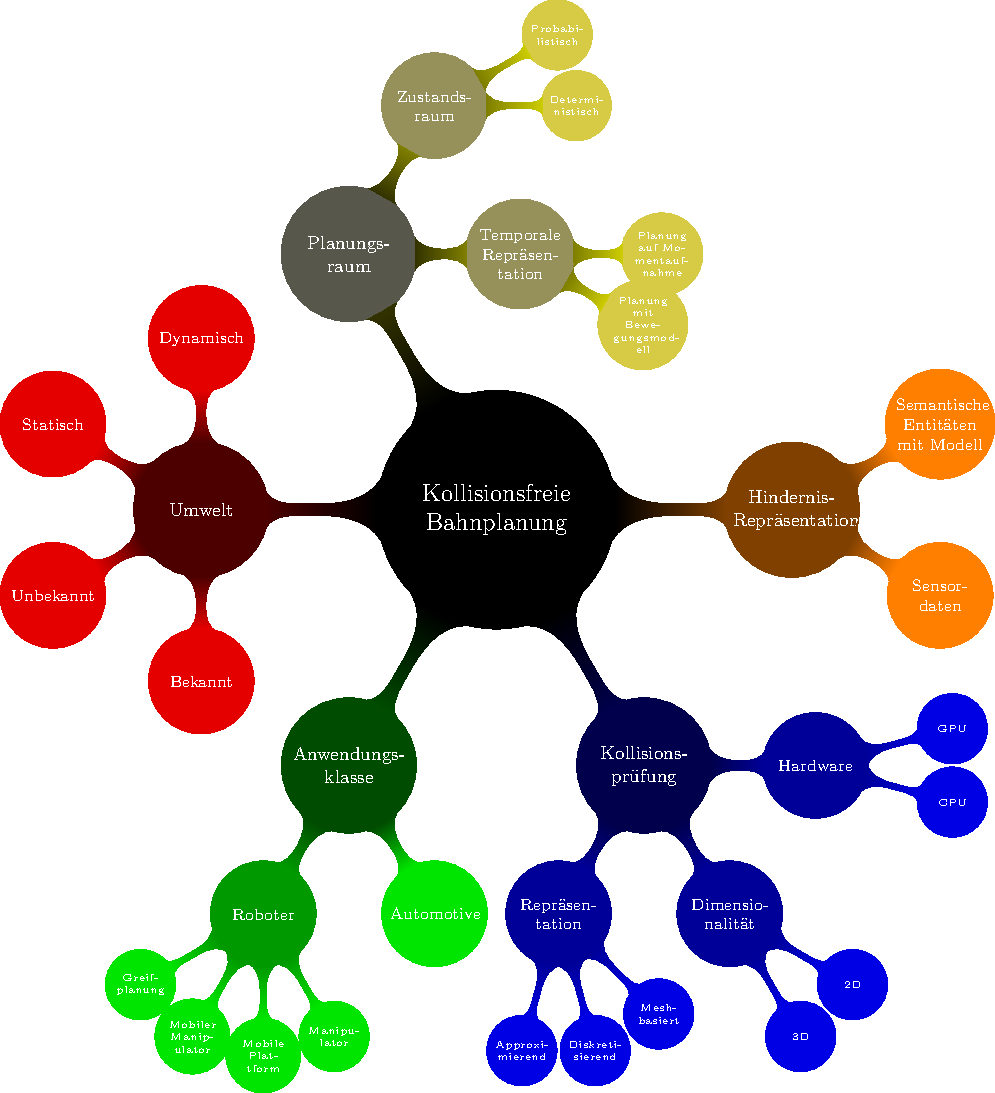
\includegraphics[width=1\textwidth]{04_images/sota_taxonomy}

Notes from the "Combine PhD with projects workshop with Arne and EG with Marius from 06/2021:
\begin{enumerate}
    \item Huge "snow-Balling" leads to very many sources (not so good)
    \item If research shows cross-references ("Oh, I read this paper before") this is a good point to stop
    \item SotA Freeze shortly before finishing, also recent sources should be included
    \item How to deal with recent publications that have "overtaken" this work? Put those after the own methods later in the document and state "my method can be further improved as shown in" in the outlook. More difficult, if a later publication is 10x better than my own work and crushes it.
    \item JMZ likes the work of Breitenstein
    
\end{enumerate}

Beispiel für ein ordinäres Zitat:~\cite{Schwarzer05adaptivedynamic}.

Beispiel für das Zitat einer eigenen Arbeit:~\citeownpubs{Hermann2014_ISR}.

Beispiel für das Zitat einer Studentischen Arbeit:~\citestudthesis{drews14}.

\section{General definition of corner cases}

See first PhD seminar
\begin{enumerate}
    \item rare event
    \item corner case
    \item edge case
    \item unusual event \cite{bolte_towards_2019}
    \item anomaly detection \cite{bolte_towards_2019}
    \item novelty detection \cite{bolte_towards_2019}
\end{enumerate}

\section{Definition of corner cases in the context of autonomous vehicles}

\todo{Knowledge-driven vs data-driven}

While the term \emph{corner case} is mentioned in the context of autonomous driving several times in the literature\todo[]{Find and cite literature before 2019}, no formal definition of its meaning was attempted until 2019, when Termöhlen (previously Bolte) et al. stated the following:

\begin{displayquote}[\cite{bolte_towards_2019}]
A corner case is given, if there is a non-predictable, 
relevant object/class in [a] relevant location.
\end{displayquote}

This definition is motivated by the task of detecting corner cases in video data. Their proposed \emph{corner case detector} is designed as either an offline analysis tool for datasets or an online module to communicate corner cases to a \emph{autonomous driving system}. While it is very actionable, the narrow focus on relevant, "technically unpredictable situations" neglects many types of scenarios, which might be seen as corner cases.
Therefore, in follow-up publications, Breitenstein et al. buildt upon the results and introduced a broadened \emph{Systematization of Corner Cases} in \cite{ breitenstein_systematization_2020} and extended it in \cite{breitenstein_corner_2020}, as shown in fig. \ref{fig:systematization_corner_case}.

\begin{figure}[hbtp]
\centering
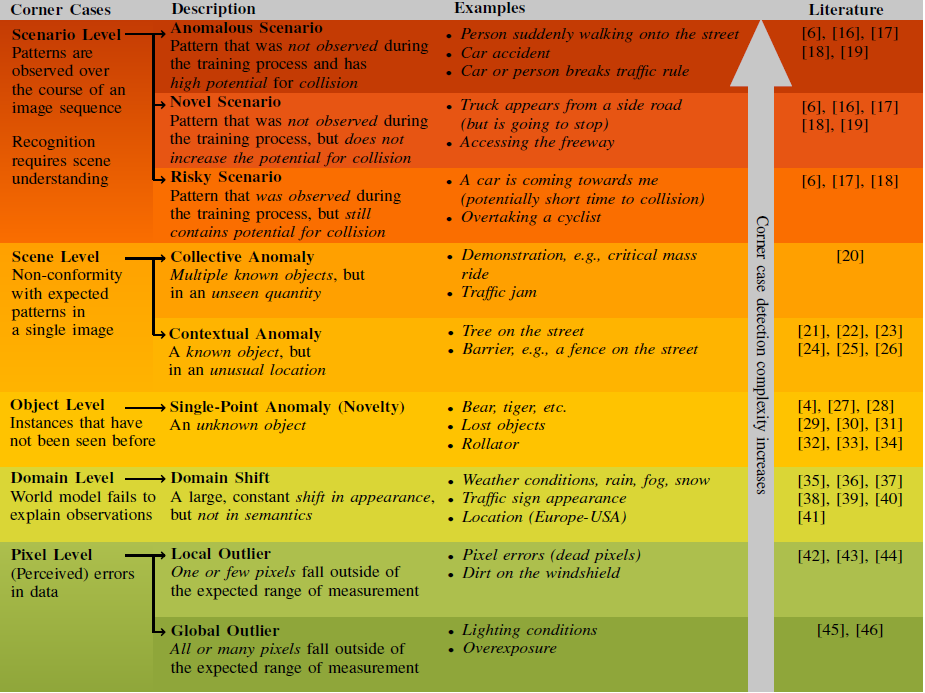
\includegraphics[scale=1]{04_images/sota/corner_cases_systematization.png}
\caption{"Systematization of corner cases on different levels"\cite{breitenstein_systematization_2020}}
\label{fig:systematization_corner_case}
\end{figure}

\begin{displayquote}[IESChat, Jasmin Breitenstein, 24 June 2021]
Wir haben die dann zusammen erweitert zu der Systematisierung, weil die bisherige Definition nicht alles abgebildet hat, vor allem nicht unser Bild, dass verschiedene Arten von CoCas verschiedene Detektionsmethoden brauchen
\end{displayquote}

Extended to typical AD-sensor stack (camera, radar, lidar) by \cite{heidecker_application-driven_2021}.

Different approaches from the same domain:

\begin{displayquote}[\cite{houben_inspect_2020}]
Inputs that result in unexpected or incorrect behaviour \end{displayquote}

\begin{displayquote}[\cite{hanhirova_machine_2020}]
Rare combinations of input parameter values \end{displayquote}

\begin{displayquote}[\cite{chou_using_2018}]
By an interesting corner case, we mean
initial conditions from which ensuring safety is hard but not
necessarily impossible 
\end{displayquote}

\begin{displayquote}[\cite{hesse_potenziale_2021}]
Trotzdem verbleibt ein Restrisiko für mögliches Fehlverhalten. Dieses tritt häufig im Zusammenhang mit sogenannten Edge und Corner Cases (Grenz- und Übergangsfälle) auf. Diese beschreiben Sonderfälle, die so selten auftreten, dass die Lernenden Systeme dafür gegebenenfalls nicht ausreichend konzipiert, trainiert und getestet wurden.
\end{displayquote}

Issue: Current cc detectors work with metric, so a system can known "that something is wrong" but it can hardly know "what is wrong". Therefore, machine-interpretable corner case description is necessary.

\section{Knowledge- and data-based descriptions of corner cases}

\section{Vision and multi-modal based detection of corner cases}

\section{Machine-learning based planning methods and their handling of corner cases}





\cleardoublepage
\chapter{Description of Corner Cases}
\label{chap:description}

\section{Machine-interpretable corner case descriptions}
\label{sec:sensorik}

\section{Evaluation}


\cleardoublepage
\chapter{Detection of Corner Cases}
\label{chap:detection}

\begin{enumerate}
    \item JMZ would also like "novel scenarios" from Breitenstein (EG 06/2021)
\end{enumerate}

\section{Multi-modal detection of corner cases}
\label{sec:sensorik}

\section{Evaluation}


\cleardoublepage
\chapter{Handling of Corner Cases}
\label{chap:handling}

\section{Handling of corner cases based on informaed machine learning}
\label{sec:sensorik}

\section{Evaluation}


\cleardoublepage
\chapter{Evaluation}
\label{chap:evaluation}

\section{Some evaluation stuff}

Notes of EG with JMZ 06/2021

\begin{enumerate}
    \item Systematic of the evaluation:
    \item What do I evaluate? Want to show that Perception/Handling works.
    \item Sim2Real (nvidia and Intel Papers for perception)
    \item JMZ want at least demonstration on CoCar (1 Component, variations of 1 scenario). I think either perception (in KIGLIS?) or something which affects the planner (driving area based on KI-W?)
    \item Generator that generates scenarios in CARLA. Then argue the selection (e.g. samples for scenarios in categories). Alright if it's not complete (see EG 07/2021 skizze ppt, scenario based evaluation)

\end{enumerate}

\cleardoublepage
\chapter{Conclusion}
\label{chap:extro}


\section{Summary of Contributions}

\section{Open Problems}

\section{Discussion}

\section{Outlook}

\cleardoublepage
% ...

\appendix
\renewcommand*{\thechapter}{\Alph{chapter}}
\addpart{\appendixname}
%\chapter{Appendix 1}
\label{chap:appendix1}


\section{Partikelschwarmoptimierung}
\label{appendix:pso}
Die Partikelschwarmoptimierung ist ein biologisch motiviertes Optimierungsverfahren, das 1995 durch Kennedy et al. vorgestellt \cite{Kennedy1995}.
Es bildet das Verhalten eines Schwarmes nach, dessen Individuen bzw. Partikel $n$ einerseits eigenständig nach einem Optimum suchen, und andererseits durch das Verhalten des erfolgreichsten Schwarm-Individuums $b$ beeinflusst werden.
Dabei wandert jedes Partikel mit einer sich verändernden Geschwindigkeit $\vec{v}_n$ durch den Suchraum $X$ des Optimierungsproblems und speichert dabei seine bisher beste erreichte Position $\vec{x}_{n\,\text{best}}$.
Da der Schwarm ein randomisiert exploratives Verhalten aufweist, können lokale Minima bei passender Parametrierung vermieden werden.
In dieser Arbeit wird die PSO dafür genutzt, nichtlineare Optimierungsprobleme anzugehen.
Dafür gilt:

Maximiere die Bewertungsfunktion $f(\vec{x})$ unter der Nebenbedingung $\vec{x}\in X$ mit $f\colon W\to \mathbb{R}$ eine reellwertige Funktion und $X \subseteq W$. 
Die zulässige Menge $X$ ist durch ihren konkreten Wertebereich beschrieben.

Die Implementierung iteriert nach einer Initialisierung durch drei Phasen, bis ein Maximum an Iterationen erreicht ist, oder ein Abbruchkriterium für das Ergebnis von $f(\vec{x})$ erreicht wurde.

Zunächst wird ein Schwarm mit einer festen Anzahl $N$ an Partikeln erzeugt, indem jedem Individuum $n \in N$ ein randomisierter Startwert $\vec{x}_n$ zugewiesen wird.
Danach startet die Optimierung:
\begin{enumerate}
	\item Bewerte: Berechne $f(\vec{x}_n)$ für alle $n$ und setze $\vec{x}_{n\,\text{best}}$, falls $f(\vec{x}_n) > \vec{x}_{n\,\text{best}}$
	\item Ermittle Schwarm-Besten $\vec{x}_b = \argmax_{n \in N} (f(\vec{x}_n))$ aus allen $N$ Partikeln
	\item Berechne neue Partikel-Geschwindigkeit: \\
	$\vec{v}_n = \vec{v}_n 
	+ \big( \alpha \cdot p_1 \cdot (\vec{x}_{n\,\text{best}} -  \vec{x}_n ) \big) 
	+ \big( \beta \cdot p_2 \cdot (\vec{x}_b - \vec{x}_n) \big)$ \\
	mit Zufallsvariablen $p_1, p_2 \in [0, 1]$
	\item Verschiebe Partikel: $\vec{x}_n = \vec{x}_n \cdot \vec{v}_n$
\end{enumerate}
Dabei kann über die Parameter $\alpha$ und $\beta$ gesteuert werden, wie stark Partikel von ihrem eigenen Optimum $\vec{x}_{n\,\text{best}}$ oder dem Schwarm Optimum $\vec{b}$ angezogen werden.
Durch die Zufallsvariablen $p_1$ und $p_2$ streut der Schwarm und konvergiert nicht direkt gegen ein einziges Maximum.
Analog kann über entsprechende Umstellungen $\text{max} \to \text{min}$ auch ein Minimierungsproblem gelöst werden.



%\chapter{Appendix 2}
\label{chap:appendix_gpu_voxels}

\begin{figure}[hbtp]
\centering

\includegraphics[scale=1]{04_images/gpu_voxels_logo_small.png}
\caption{Logo der GPU-Voxels Bibliothek, das die Würfelstruktur andeutet}
\label{fig:gpu_voxels_logo}
\end{figure}

ROS Universum und OctoMap

OpenSource Bibliothek

UML Diagramme von
\begin{itemize}
\item GPU-Voxels (Octree)
\item Visualisierung
\end{itemize}

Pseudocode von
\begin{itemize}
\item Prädiktion
\item Load-Balancer
\end{itemize}

\cleardoublepage
\backmatter

\newpage
\improvement[inline]{Alle Tabellen zu Booktabs machen}
\improvement[inline]{Mit ack-grep alle refs und cites auf geschützte Leerzeichen testen}
\change[inline]{Kommazahlen in allen Tabellen prüfen. Komma statt Punkten.}

\listoftodos[Notes]

\listoffigures
\listoftables

% use the following two lines with natbib
%\bibliographystyle{alpha}
%\bibliography{fzi_references_ah,general_references_ah}

% use this line with biblatex:
% \printbibliography


\renewcommand{\bibpreamble}{Dieses Verzeichnis listet alle Publikationen, bei denen der Autor dieser Dissertation entweder der Erstautor ist, oder als Co-Autor maßgeblich zu der Veröffentlichung beigetragen hat (in Form von Problemstellung, -lösung, Diskussion oder experimenteller Evaluation).}
\nociteownpubs{*}
\bibliographystyleownpubs{plain}
\bibliographyownpubs{05_bib/own_publications_ah}

\renewcommand{\bibpreamble}{Dieses Verzeichnis listet studentische Arbeiten, die durch den Autor dieser Dissertation im Rahmen seiner Forschung ausgeschrieben und betreut wurden. Dies beinhaltet die maßgebliche Vorgabe der Problemstellung, Diskussion der Arbeit, sowie Randvorgaben zur Lösung, Visualisierung und experimentellen Evaluation.}
\nocitestudthesis{*}
\bibliographystylestudthesis{plain}
\bibliographystudthesis{05_bib/student_references_ah}

\renewcommand{\bibpreamble}{}
\bibliographystyle{plain}
%\bibliography{05_bib/fzi_references_ah,05_bib/general_references_ah}
\bibliography{05_bib/zotero}

\printindex

%% Your CV should be included in the dissertation
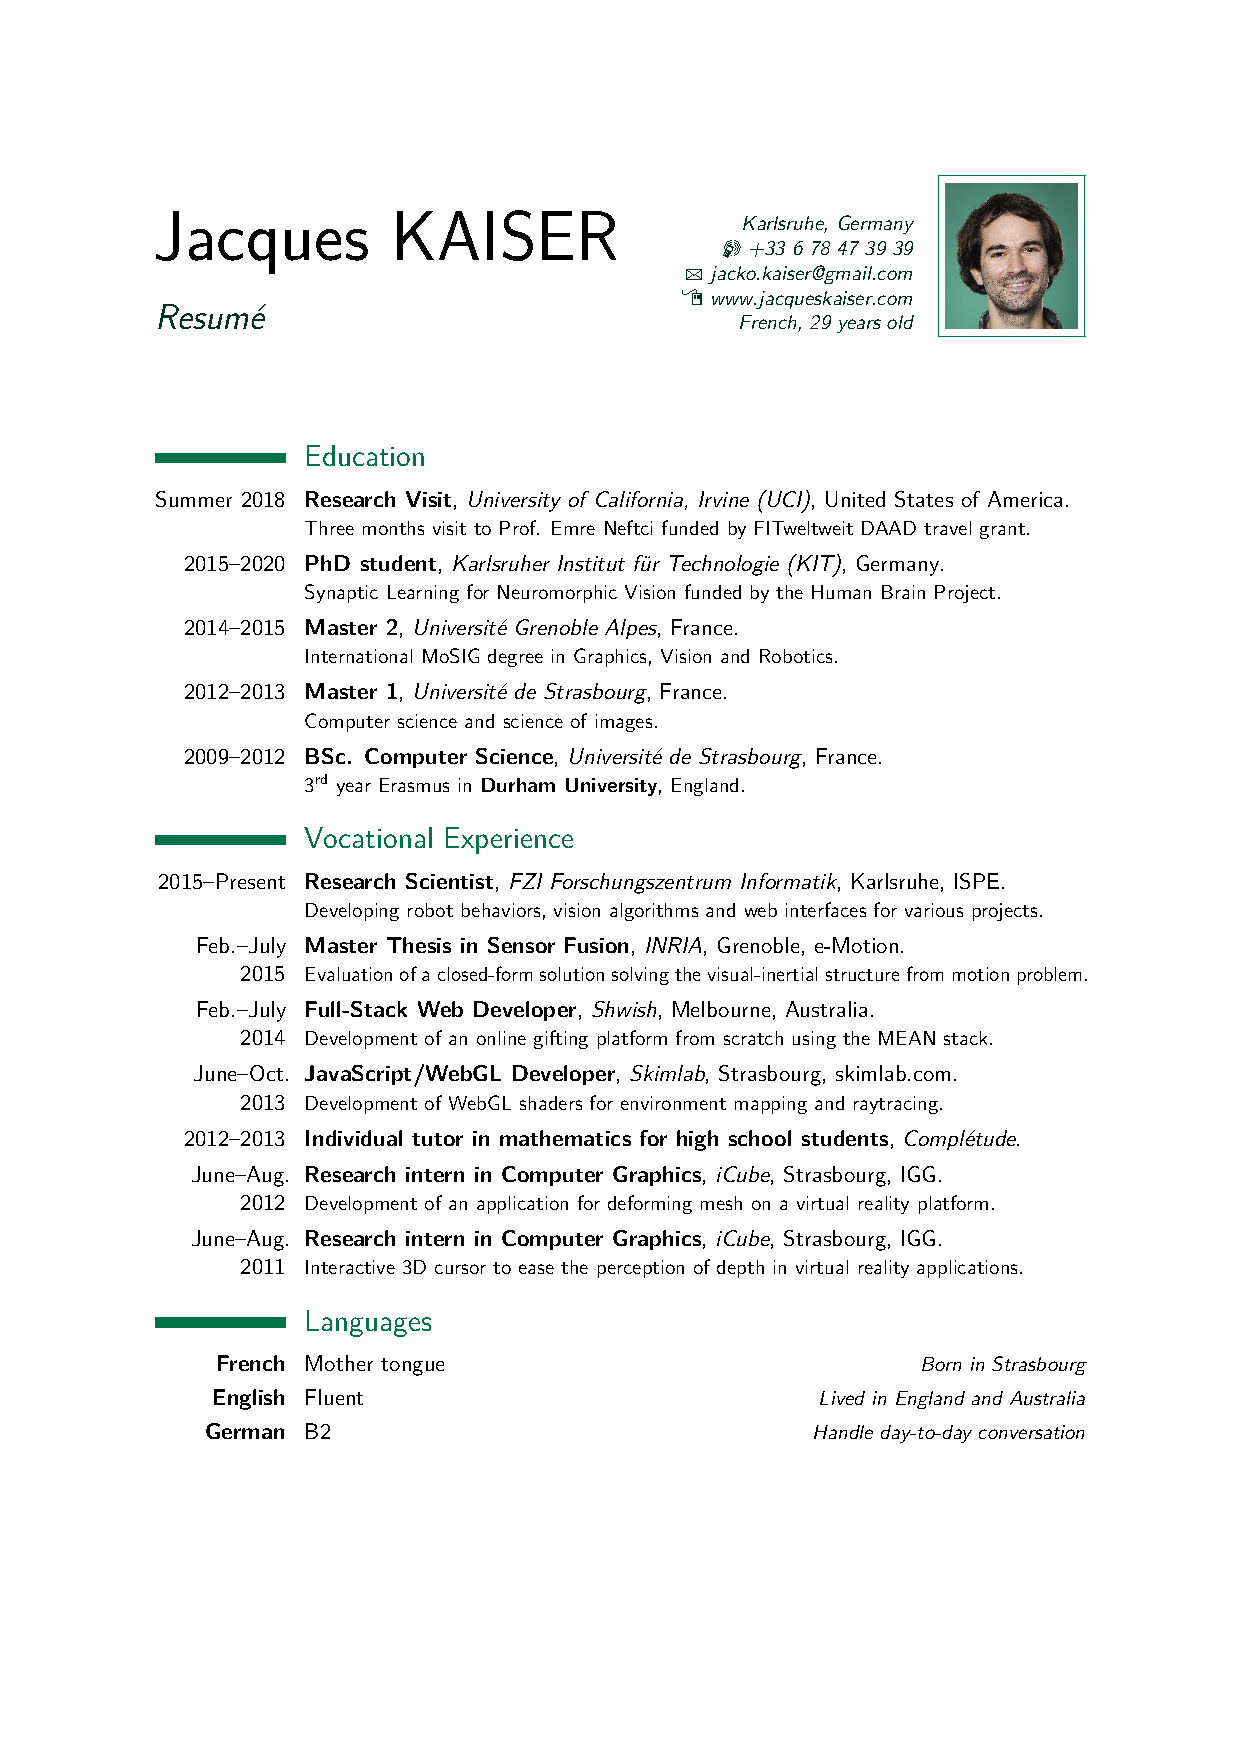
\includepdf[pages=1-]{03_content/cv.pdf}

\end{document}
